\section{Prototipo (Aplicaci�n)}
\begin{frame}%[allowframebreaks]
	\frametitle{Prototipo (Aplicaci�n)}
	%%%%%%%%%%%%%%%%%%%%%%%
	\begin{block}{Dificultad}
	\justifying 
	La b�squeda y recuperaci�n en un modelo sem�ntico no son actividades sencillas, porque se requiere que un usuario tenga conocimientos en el 
uso de las tecnolog�as sem�nticas y los vocabularios en las ontolog�as.
	\end{block}
	
	\begin{block}{Prototipo}
	\justifying 
	Una aplicaci�n Web para que los usuarios puedan consultar y visualizar la informaci�n de los \textit{recursos de informaci�n}, mediante una ontolog�a (Redes y Telecomunicaciones).
	\end{block}
	
	\begin{block}{Prototipo}
	\begin{itemize}
	\item \justifying Navegaci�n entre informaci�n de los \textit{recursos de informaci�n}.
	\item \justifying B�squeda Avanzada de los \textit{recursos de informaci�n}.
	\item \justifying Detalles de un \textit{recurso de informaci�n}.
	\end{itemize}
	\end{block}
\end{frame}

\begin{frame}%[allowframebreaks]
	\frametitle{Navegaci�n entre informaci�n de los recursos de informaci�n}
	\begin{figure}
	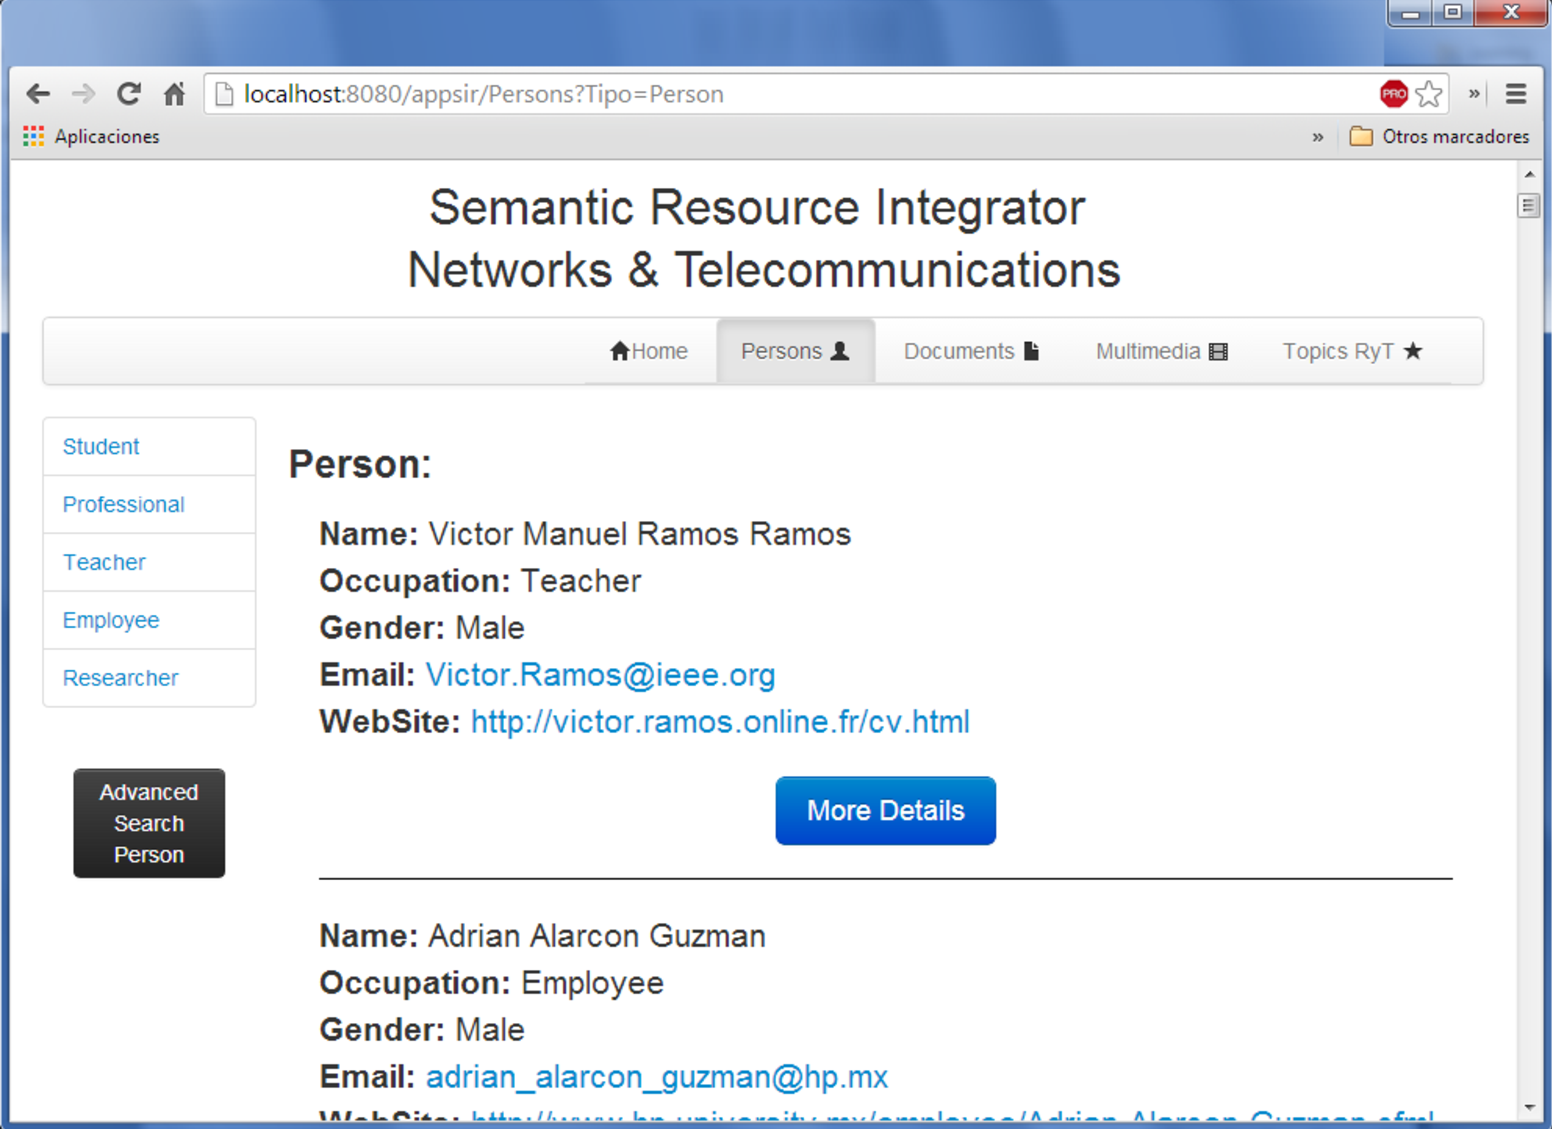
\includegraphics[scale=0.35]{IntWebNavPer} 
	\end{figure}
\end{frame}

\begin{frame}%[allowframebreaks]
	\frametitle{B�squeda Avanzada de los recursos de informaci�n}
	\begin{figure}
	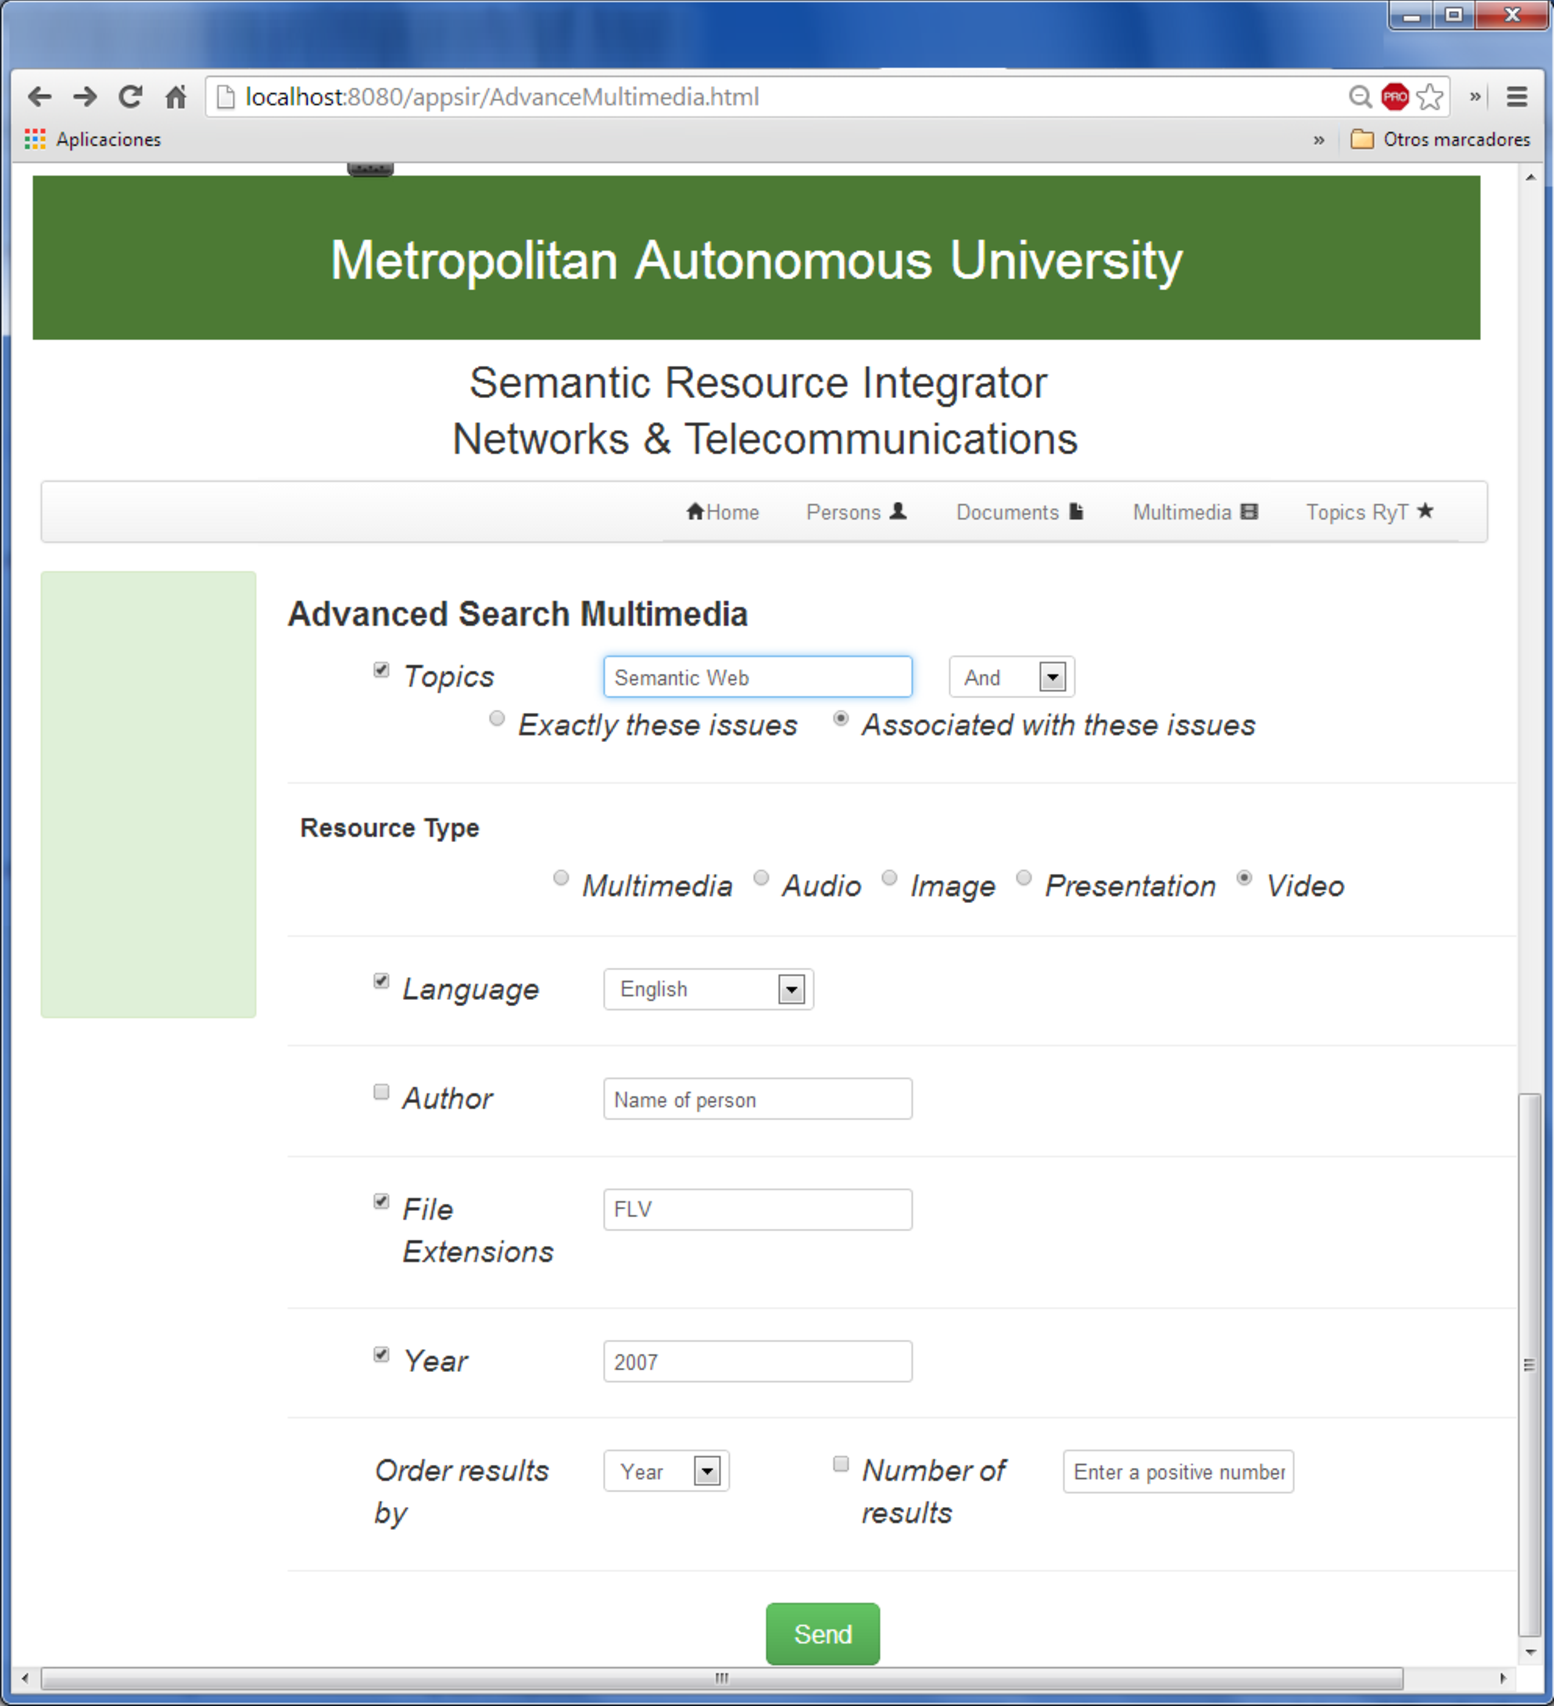
\includegraphics[scale=0.23]{FormBusMult} 
	\end{figure}
\end{frame}

\begin{frame}%[allowframebreaks]
	\frametitle{Detalles de un recurso de informaci�n}
	\begin{figure}
	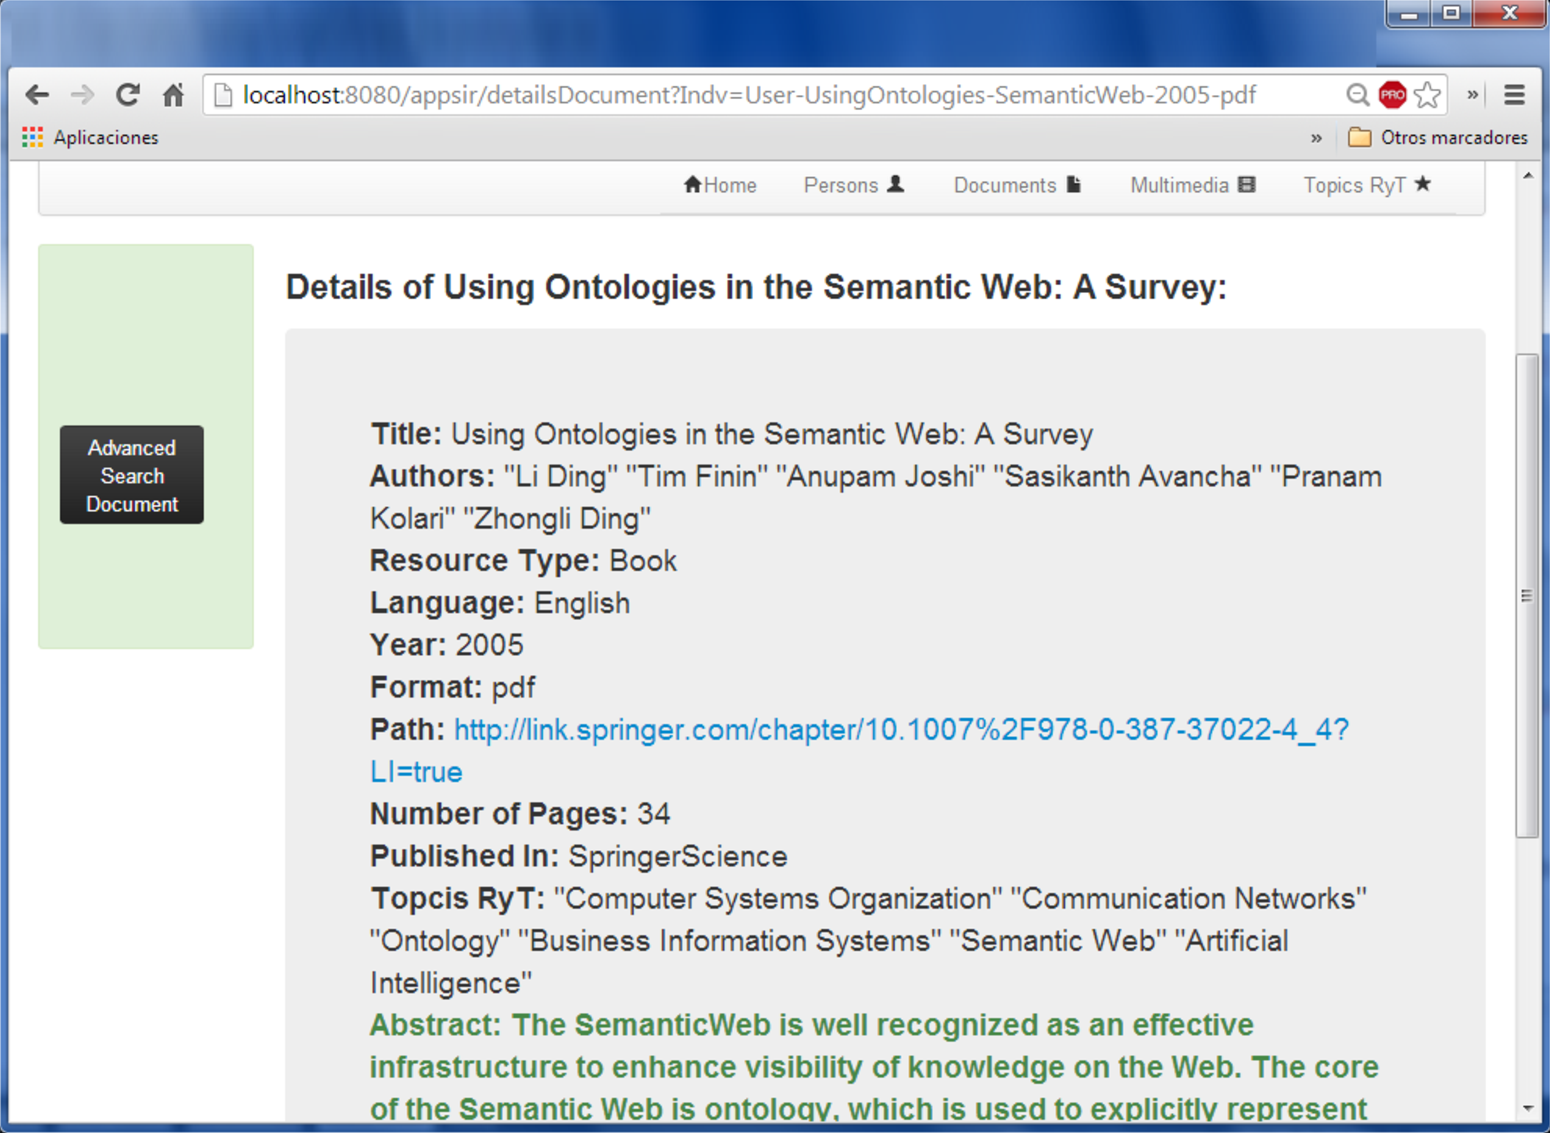
\includegraphics[scale=0.35]{IntWebDetDoc} 
	\end{figure}
\end{frame}